\documentclass{article}
\usepackage{indentfirst}
\usepackage{polski}
\usepackage[utf8]{inputenc}
\usepackage{sidecap}
\usepackage{wrapfig}
\usepackage{graphicx}
\usepackage{hyperref}

\marginparwidth = 70pt
\oddsidemargin = 30pt
\textwidth = 400pt

\title{
Nikola Tesla -\\- czyli historia człowieka, wizjonera, \\o którym zapomnieliśmy, nie doceniliśmy,\\a wiele mu zawdzięczamy.}
\author{Mateusz Knoblauch}

\begin{document}

\begin{Huge}
\maketitle
\end{Huge}


\newpage


\begin{center}

\tableofcontents

\ldots{}

\end{center}


\newpage

\begin{Huge}
\section{Wstęp}
\end{Huge}

\begin{large}

Niewiele dzisiaj pisze się o dokonaniach ludzi żyjących przeszło sto lat temu. Szczególnie mało wspominamy o ludziach, których dokonania ostatnio są tematem dyskusji tylko i wyłącznie ciasnego i zamkniętego grona . Ile to "zwykłych" ludzi interesuje się fizyką w takim stopniu, by rozpamiętywać dochodzenie uczonego do pewnych wniosków, które są poprzedzane (dla wielu) przez skomplikowane wzory matematyczne i fizyczne? Tylko niewielka część z nas ma tyle chęci, by zagłębić się w historię, opowiadania, domniemania, by później dojść do własnych wniosków i spostrzeżeń. Coraz rzadziej spotykana jest dziecięca ciekawość połączona z  zadawaniem pytań: "Jak? Dlaczego?" Dziecko szuka odpowiedzi, chce znać naturę wszechrzeczy która je otacza. Coraz mniej ludzi zachowuje tę cechę charakteru w miarę upływu lat.
\\
\\

\indent Oto krótkie opracowanie, które stanowi część wiedzy o dorobku naukowym, jaki pozostawił po sobie Nikola Tesla. Zebrałem informacje, które według mnie były warte uwagi i złożyłem, tworząc historię, którą każdy powinien poznać.

\indent Zapraszam do lektury!

\end{large}


\newpage


\section{Od dziecka, do wizjonera.}


\begin{large}


\subsection{Dzieciństwo}
\begin{wrapfigure}{l}{0.5\textwidth}
\vspace{0pt}
\includegraphics[scale=0.24]{Nikolahome.jpg}
\vspace{-10pt}
\caption{Dom Nikoli w Smiljanie}
\vspace{-10pt}
\end{wrapfigure}


Nikola Tesla urodził się o północy z 9-10 lipca 1856 roku, w małym miasteczku w Smiljanie na terenie Chorwacji (ówczesne  terytorium imperium Austro-Węgierskie). Sama chwila narodzin Tesli była niezwykła, bo w noc jego narodzin rozpętała się burza. Można by powiedzieć, że od samego początku swojego życia miał bliską styczność z elektrycznością. O jego dzieciństwie wiemy niewiele. Jego matka była niezwykle uzdolnioną kobietą, która produkując tekstylia przędła najpiękniejsze wzory. Cały czas, własnoręcznie, udoskonalała swoje narzędzia pracy. Była równie genialna jak Nikola, ale jeszcze bardziej uzdolniony od Nikoli był jego brat - mówił o nim później: umysłowy gigant. Jednakże jego brat zmarł w młodzieńczym wieku podczas upadku z konia. Tesla do końca życia obwiniał siebie o śmierć brata, mówiąc że to była jego wina.
\cite{art:1}
\\


\subsection{Edukacja}

\begin{wrapfigure}{r}{0.5\textwidth}
\vspace{-20pt}
\includegraphics[scale=0.55]{Tesla_at_19.jpg}
\vspace{-10pt}
\caption{Nikola w wieku 19 lat}
\vspace{-10pt}
\end{wrapfigure}

\indent Swoją edukację Nikola rozpoczął po przeprowadzce do Gospić'a, w Karlovac, którą ukończył w zaskakującym czasie 3 lat. W wieku 12 lat opanował na pamięć tablice logarytmiczne i zaczął konstruować swoje własne silniki, które różniły się całkowicie od tych, które mogłoby się zobaczyć w okolicy. Jego ojciec, który był ortodoksyjnym kapłanem kościoła serbskiego, chciał by jego syn podążył w jego ślady. Ojciec nie uznawał pomysłu wysłania swojego syna na studia. Młody Tesla zachorował przy tym na cholerę niemal ocierając się o śmierć. Oznajmił swojemu ojcu, że być może będzie czuł się lepiej, kiedy pozwoli mu studiować. Po namowie miejscowego nauczyciela i wystaraniu się przez niego o stypendium dla Nikoli, ojciec zmienił zdanie.
\\

\indent W 1875 roku Tesla rozpoczął naukę na Politechnice Austriackiej w Gratzu na kierunku: inżynieria energetyczna. To umożliwiło mu poważne rozważania i realizację swoich projektów o wykorzystywaniu źródeł alternatywnych do pozyskiwania energii. Po matce odziedziczył pamięć wzrokową, dzięki której bardzo szybko opanował aż 6 języków, a jego wyliczenia "na oko" miały margines błędu rzędu jednej dziesięciotysięcznej jednostki podstawowej. Był bardzo ambitny, potrafił siedzieć nad książkami po 20 godzin dziennie, byleby tylko ukończyć rozważanie interesującego go zagadnienia. Prowadził spór o wyższość prądu zmiennego nad stałym oraz wykorzystania go do napędu silników elektrycznych. Profesor podsumował jego stwierdzenie przy wszystkich w grupie, że jest to pomysł godny perpetuum mobile, zupełnie niemożliwy do wykonania. Ten sam profesor pomógł mu później uzyskać posadę telegrafisty w biurze telegraficznym w Budapeszcie.

\indent Po likwidacji urzędu telegraficznego oraz opuszczeniu uczelni (stwierdzając, że przewyższył poziomem wszystkich swoich wykładowców) Nikola Tesla przybył do Paryża, by rozpocząć pracę w Continental Edison Company - przy tym wszystkim zerwał również kontakt z rodziną. Tak, była to słynna korporacja Thomasa Alva Edisona, która we francuskim oddziale produkowała prądnice, silniki prądu stałego i oświetlenie chronione patentami Edisona. Zgodnie z zapisami, po naprawie instalacji elektrycznej na stacji kolejowej w Strasburgu ratując dobre imię firmy nie otrzymał zapłaty, postanowił złożyć wypowiedzenie i wyjechać do Stanów Zjednoczonych, by osobiście spotkać się z Thomasem Edisonem.
\cite{art:2}

\newpage


\subsection{Początek rywalizacji}

Tesla przybył do Nowego Jorku 6 czerwca 1884 roku. Wysiadając ze statku posiadał w kieszeni ostatnie 4 centy. Na tę podróż wydał wszystkie oszczędności. Miał ze sobą niewiele, posiadał tylko list polecający od Charlesa Betchelora do Thomasa Edisona z treścią:
\\

\begin{verbatim}
"Znam dwóch wielkich ludzi, a Ty jesteś jednym z nich.
Drugim jest ten o to młody mężczyzna."

\end{verbatim}

\begin{wrapfigure}{r}{0.6\textwidth}
\vspace{-5pt}
\includegraphics[scale=0.4]{turbiny.jpg}
\vspace{-15pt}
\caption{Turbiny w laboratorium T. Edisona}
\vspace{-10pt}
\end{wrapfigure}

\indent Tesla był zafascynowany fabryką i laboratorium Edisona, jednak Edison nie był zadowolony z pomysłów Tesli. Produkcja oświetlenia i silników na prąd stały w Nowym Yorku trwała nieprzerwanie od 1870 roku. Nikomu w tych czasach nie przeszkadzało, że miasto splątane było tysiącami przewodów, a generatory prądu musiały znajdować się prawie na każdej ulicy. Nie dało się za pomocą prądu stałego wysłać energii elektrycznej dalej niż na kilkaset metrów od elektrowni! Nie było to wygodne, ale w owych czasach było to jedyne rozwiązanie na rozświetlenie żarówek lub uruchomienie elektrycznych tramwajów.

\indent Edison chwalił prąd stały i prostotę jego zastosowania. Silnik prądu stałego wymagał tzw. szczotek (komutatorów), by przesłać energię elektryczną do twornika. Poprzez snop iskier silnik obracał się dając energie kinetyczną. Tesla zaproponował usprawnienia. Chciał, by Edison pomógł mu rozwiązać problem z prądem zmiennym, który dał się transmitować na wielkie odległości bez większych strat. W owych czasach przejście na prąd zmienny było niemożliwe, ponieważ nie istniał silnik, który mógłby odebrać taką energię, a Tesla miał pomysł na jego budowę. Pomimo irytacji Edisona prądem zmiennym, zaproponował Tesli posadę. Obiecał, że zapłaci 50 tyś dolarów (co było w tych czasach znaczną kwotą), za wprowadzenie usprawnień do istniejącego systemu. Po ponad rocznej pracy nad usprawnianiem silnika prądu stałego, Tesla ukończył pracę i zażądał zapłaty. Edison wyśmiał go i powiedział, że nie zna się na amerykańskim poczuciu humoru. Tesla miał dość pracy z Edisonem i odszedł.
\cite{art:3}

\subsection{Nierówna walka}

\indent Przez kolejny rok Tesla pracował fizycznie, kładąc przewody w korporacji Edisona. Cały czas myślał o konstrukcji silnika prądu przemiennego. Wraz ze znajomymi otworzył kilka przecznic od biura Edisona własne laboratorium. Przez 7 lat pomysł silnika znajdował się tylko w głowie Tesli. Teraz miało się to zmienić. Tesla rozpoczął pracę nad prototypem. Badał możliwości tworzenia prądu przemiennego, jego transmisji i odbioru w postaci żarówek i silnika. Tworzył podstawy prądu zmiennego, który płynie w naszych domach po dziś dzień. W 1888 roku Tesla pokazał światu swój pierwszy silnik na prąd zmienny. Otrzymał pierwsze patenty.



\begin{wrapfigure}{l}{0.65\textwidth}
\vspace{+5pt}
\includegraphics[scale=0.29]{silnik.jpg}
\vspace{0pt}
\caption{Patent silnika elektrycznego Tesli v. AC}
\vspace{-0pt}
\end{wrapfigure}


\indent Nowy silnik miał wiele zalet nad silnikiem Edisona. Nie wymagał przenoszenia prądu elektrycznego za pomocą komutatora. Silnik obracała siła pola elektromagnetycznego, jednak Tesla opatentował zasadę ustawienia cewek w silniku i odpowiednie wykorzystanie zjawiska prądu przemiennego. O tym co w oczach profesora i innych było perpetuum mobile, w 1888 roku okazało się możliwe i doskonałe w swej prostocie i wydajności. Tesla wykonał również własną żarówkę, jednak nie mógł wykorzystać patentu Edisona na standardowy gwint w żarówce. Opracował zatem własną żarówkę, zakończoną dwoma bolcami przez które płynął prąd.

\indent Edison widząc co się dzieje, rozpoczął tzw. wojnę prądową, wskazując niebezpieczeństwa jakie daje prąd zmienny. Demonstracyjnie pokazywano uśmiercanie zwierząt prądem zmiennym. Straszono, że prąd zmienny jest niebezpieczny dla zdrowia i życia ludzi. W dalszych pracach nad rozwojem prądu zmiennego Tesli pomagał słynny wynalazca i przedsiębiorca George Westinghouse. Dzięki niemu zbudowano sieć elektrowni i oświetlono wszystkie stacje Western Union świetlówkami Tesli. Edison walcząc o dobre imię prądu stałego, zaproponował krzesło elektryczne na prąd zmienny. Pierwszy skazaniec miał być tzw. \emph{Westinghousowany} – uśmiercany szkodliwym prądem zmiennym. Oczywiście były to tylko próby pokazania jak bardzo niebezpieczny jest prąd zmienny, nie pokazując eksperymentów na prądzie stałym. W późniejszych czasach rząd USA przerwał wojnę Tesli z Edisonem, nakazując Edisonowi przejście na prąd zmienny i zastosowanie urządzeń i patentów Nikoli Tesli.

\newpage


\section{Nowy rozdział w historii technologii świata}


\subsection{Wizjoner}


\begin{wrapfigure}{l}{0.56\textwidth}
\vspace{-10pt}
\includegraphics[scale=0.23]{lab.jpg}
\vspace{0pt}
\caption{Tesla w laboratorium.}
\vspace{0pt}
\end{wrapfigure}

Tesla był pionierem bezprzewodowego przesyłu energii, skonstruował pierwszy zdalnie sterowany pojazd, lecz Nobla za radio otrzymał Guglielmo Marconi\cite{art:6}, wykorzystując 17 patentów Tesli... w 1943 roku sąd po wieloletnich rozprawach ogłosił że Marconi wykorzystał patenty Tesli, jednakże już pośmiertnie i po dorobieniu się przez Marconiego fortuny. W 1887 Tesla pracował nad promieniowaniem, które lata później nazwano promieniowaniem x. Wykonał pierwsze zdjęcie kości swojej dłoni i wysłał je do Wilhelma Roentgena... Teoretyczny wkład w poznanie właściwości fal niezbędnych do określenia położenia i prędkości ruchomych obiektów, zostały 5 lat później wykorzystane przez Taylora i Younga - twórców radaru. Zbudował zamknięte szklane kolby z gazem, który emitował światło gdy przechodziła przez nie energia, co odkryli później twórcy świetlówek. Opisał podstawy uzyskiwania niskich oporów w niskich temperaturach 11 lat przed Noblem dla Onnesa za nadprzewodnictwo.
\cite{art:4}
\indent Opracował też rotujące pola magnetyczne, indukcyjny silnik prądu przemiennego, alternatory wysokich częstotliwości, bezprzewodowy przesył energii, cewkę bifilarną, telegeodynamikę, generator wyładowań koronowych, pompę Tesli, bezłopatkową turbinę Tesli, cewkę Tesli, zapłonową cewkę Tesli, kompresor Tesli, samolot pionowego startu i wiele wiele innych.
Nikola Tesla nigdy nie otrzymał Nagrody Nobla.
\\
Kilka ważnych wzorów sformułowanych na potrzeby zrozumienia natury prądu przemiennego:
\\
$$
Oto\ one : \left\| \begin{array}{l}
P = I \cdot U \cdot \cos{\phi}\\
\textrm{gdzie: $P$ - moc elektryczna, $I$ - natężenie prądu,}\\
\textrm{$U$ - napięcie, $\cos{\phi}$ - przesunięcie fazowe}\\
\epsilon = \frac{W}{q}\\
\textrm{gdzie: $\epsilon$ - moc elektr.mot., $W$ - praca, $q$ - ładunek elektr.}
\end{array} \right.
$$
\cite{art:5}
\indent Tesla był nie tylko genialnym inżynierem o wybitnej intuicji. Był także wizjonerem, często nie rozumianym w jego czasach. Jego wizje były tak dalece przyszłościowe, że na pewnym etapie stał się wręcz archetypem szalonego naukowca, co w połączeniu z jego licznymi dziwactwami narobiło mu sporo złej sławy i przyćmiło prawdziwe dokonania. 100 lat temu Tesla pisał słowa przyprawiające dzisiaj o dreszcze na myśl o nadnaturalnej intuicji tego człowieka:

\begin{verbatim}
"Wojny będą trwały, dopóki nie zniknie fizyczna przyczyna ich
nawrotów, którą jest w ostatecznym rozrachunku rozległość planety,
na której żyjemy. Jedynie usunięcie dystansu w każdej dziedzinie -
transmisji wiedzy, transportu ludzi i zasobów oraz transportu
energii, pewnego dnia zapewni trwałość przyjaznych stosunków. 
To czego najbardziej teraz potrzebujemy, to bliższy kontakt 
pomiędzy ludźmi i społecznościami z całej Ziemi oraz zniesienie 
tego fanatycznego oddania ideałom narodowego egoizmu i dumy, 
co zawsze podatne jest pogrążyć świat w prymitywnym barbarzyństwie."

\end{verbatim}

\indent W jego czasach, gdy świat stawiał pierwsze szyby naftowe i grzebał się w węglu w pierwszych zelektryfikowanych kopalniach zasilanych jego silnikami, Tesla myślał o energii odnawialnej... Energii ze Słońca, z wnętrza Ziemi, energii pochodzącej z wykorzystania różnicy temperatur warstw oceanu oraz wykorzystaniu energii kosmicznej uderzającej o atmosferę. Wykonywał prace i eksperymenty na wszystkich tych polach i był wręcz opętany przez ideę darmowej energii dostępnej dla każdego człowieka, w każdym miejscu na Ziemi. Darmowej w sensie odnawialnej lub  pochodzącej z przestrzeni kosmicznej.
\\
\\
Tesla zostawił też po sobie masę zagadek, hipotez, tajemnic i niewyjaśnionych eksperymentów.
\\


\newpage


\section{Eksperymenty w Colorado Springs}


\begin{wrapfigure}{l}{0.4\textwidth}
\vspace{-15pt}
\includegraphics[scale=0.42]{lab2.jpg}
\vspace{0pt}
\caption{Laboratorium Tesli.}
\vspace{0pt}
\end{wrapfigure}

Po przygodach z Edisonem, Tesla przenosi się do Colorado Springs i zakłada laboratorium. Tesla studiuje naturalne wyładowania i przeprowadza szereg eksperymentów. W swym dzienniku opisuje wytwarzanie ładunków przekraczających mocą wyładowania naturalne, 40 metrowe łuki energii, wystrzeliwujące ze szczytu budynku, o napięciu milionów volt. Przesyła energię przez atmosferę oraz samą glebę umieszczając w żarówki w gołej ziemi bez kabli i rozświetlając je na odległość wykorzystując ziemię jako przekaźnik energii. Czas spędzony w Colorado Springs, najprawdopodobniej zrodził w umyśle Tesli znacznie bardziej ambitne plany, które zamierzał wprowadzić w życie w Nowym Yorku.\cite{art:7}
\\


\subsection{Wieża Wardenclyffe}

\begin{wrapfigure}{l}{0.5\textwidth}
\vspace{-15pt}
\includegraphics[scale=1.0]{tower2.jpg}
\vspace{-15pt}
\caption{Laboratorium i wieża w C. Springs.}
\vspace{0pt}
\end{wrapfigure}


Wieża Wardenclyffe (Long Island, Nowy York), to prawdopodobnie najbardziej znany przykład wizji Tesli, której prawdziwe przeznaczenie pozostaje nie do końca jasne. Oficjalnie wieża miała pełnić funkcję nadajnika fal radiowych, do bezprzewodowego przesyłu sygnałów, głosu i zdjęć. Główny inwestor Tesli - J.P. Morgan (zgadza się, TEN J.P. Morgan), wyłożył wraz z innymi 150 tysięcy dolarów na jej budowę (dzisiejsze 3 miliony), gdy Tesla przekonał go o możliwościach przesyłu dowolnej informacji na odległość, bez użycia kabli. Tesla wiedział, że dźwięk i obraz to po prostu informacja, którą można zamienić na sygnał i nadać. Eksperymenty te wykonywał już w laboratorium, lecz wieża miała umożliwiać transfer między-kontynentalny.
\\
\\
\indent Tesla jednakże nie powiedział całej prawdy Morganowi. Transfer danych uważał już za oczywistość, natomiast sam chciał iść dalej. Z tej przyczyny wciągnął Morgana w sponsoring, obiecując pierwszą stację łączności z Europą. Miał zamiar upiec dwie pieczenie przy jednym ogniu, dając Morganowi coś co będzie mógł sprzedać, ukradkiem jednak przemycając własne koncepcje.
\\
\\

\begin{wrapfigure}{l}{0.53\textwidth}
\vspace{-15pt}
\includegraphics[scale=0.18]{tower1.jpg}
\vspace{-15pt}
\caption{"Wieża Tesli"}
\vspace{0pt}
\end{wrapfigure}

\indent Czym naprawdę miała być Wieża Wardenclyffe? Dzisiaj, po 70 latach od śmierci Tesli, nadal nie ma na to jednoznacznej odpowiedzi. Przyjrzyjmy się jednak faktom. Według źródeł, w trakcie budowy wieży, do J.P. Morgana zaczęły docierać wieści o rosnących dziwactwach Tesli, co stawiało Morgana w złym świetle. W międzyczasie w Europie doszło do pierwszego przesyłu radiowego na długi dystans, którego dokonał Marconi, tworząc własną firmę, bazującą na pracach Tesli. W tej sytuacji Morgan zaczął wątpić w Teslę, którego prace przedłużały się z powodu wdrażania ukrytych przez Teslę założeń. Morgan przycisnął Teslę do muru, grożąc wycofaniem funduszy. Tesla nie miał wyboru, postanowił zdradzić Morganowi prawdziwe przeznaczenie wieży.
\\
\\
\indent Tesla przedstawił wieżę, jako narzędzie rozsyłu energii elektrycznej, bezprzewodowo na całą kulę ziemską. Nie tylko fal radiowych, ale energii elektrycznej. Pomysł Tesli, wedle kilku źródeł, które udało mi się zlokalizować, polegał najwyraźniej na tym, aby wykorzystać jako urządzenie elektryczne CAŁĄ PLANETĘ, przewodząc elektryczność poprzez wnętrze Ziemi oraz atmosferę, wykorzystując naturalne częstotliwości rezonansowe ziemi zwane prądami tellurycznymi oraz elektryczne właściwości jonosfery, budując sieć wież, które umożliwiłyby odbiór energii elektrycznej w dowolnym miejscu na Ziemi za pomocą prostej anteny wbijanej w ziemię.
\\
\\
\indent Zanim jednak doszło do konfrontacji z Morganem , Tesla już rozpoczął swoje eksperymenty, na niedokończonej jeszcze wieży. Według kilku relacji z New York Times, świadkowie co noc widywali potężne wyładowania elektryczne wystrzeliwujące z wieży i rozświetlające noc, Tesla wykonywał również "strzelanie elektrycznością w głęboki na 50 metrów dół w ziemi", następnie gazeta spekuluje nad powodami takiego działania. Oto oryginalny artykuł opublikowany 109 lat temu :
\\

\begin{table}[t]
\begin{tabular}{|c|c|}
\hline
\includegraphics[scale=0.75]{art1.jpg} & \includegraphics[scale=0.4]{art2.jpg} \\
\hline
\end{tabular} 
\end{table}

\indent Tłumaczenie: Dziwne zjawiska w stacji Tesli


Mieszkańcy Wardencliffee, Long Island, próbują odgadnąć co tak właściwie elektryk stara się zrobić.

Cokolwiek Nicola Tesla robi w Wardencliffe, odniósł sukces w utrzymaniu wszystkiego w tajemnicy. Niektórzy twierdzą że stara się nawiązać kontakt z Marsem; inni sądzą, że wynalazł nowy system komunikacji elektrycznej przez powietrze nie używając kabli; jeszcze inni uważają, że próbuje komunikować się z domniemaną drugą stacją w Chinach lub na Syberii używając do tego Ziemi samej w sobie.

Dziwne zjawiska w pobliżu stacji Tesli w Wardencliffe są przyczyną ekscytacji mieszkańców w trakcie obserwacji eksperymentów. Nikt nie ma prawa zbliżyć się do tych wprowadzających w konsternację dzieł Tesli, a sami pracownicy nie pozostawiają żadnego komentarza. Sam naukowiec jest rzadko widywany, a kiedy zdecyduje się zabrać głos, oświadcza, że przeprowadza eksperymenty nad komunikacją bezprzewodową.

„Pewnego dnia,” - jak mówi, „ale nie dziś, wydam oświadczenie na temat czegoś, o czym nawet ja sam nie śniłem.”

Przez wiele lat Tesla był na krawędzi ogłoszenia czegoś, co miało sparaliżować cały świat. W laboratorium przy ulicy Houston posiada zagadkową maszynę, która wystrzela lśniące błyskawice w atmosferę. Wielu naukowców i finansistów przygląda się temu z zaciekawieniem.

Podobne błyskawice, dłuższe i bardziej intensywne, rozpoczynają swój bieg ze szczytu wieży Tesli w Wardencliffe. Mieszkańcy spoglądają na nie siedząc przed własnymi domami, a w przerwach pomiędzy ukąszeniami komarów spekulują na temat znaczenia dziwnych świateł, które pojawiają się, aby następnie rozpłynąć się w powietrzu.

Pod wysoką wieżą kryje się dół głęboki na 150 stóp. (ok. 45 metrów, jeśli mówimy o stopie angielskiej) Sam Tesla przyznaje, że wystrzela w głąb dziury prąd elektryczny i nie ma wątpliwości, że wytwarza błyskawice zdolne osiągnąć samo jej dno.

Wyglądający na bystrego tajemniczy człowiek, który myszkuje w pobliżu Wardencliffe, dowiedział się, że Tesla próbuje wydobyć prąd z planety nie używając żadnych sztucznych przewodników. Pewien człowiek w Chicago sądzi, że jeśli wystrzeli magnes na odpowiednią wysokość, będzie w stanie zebrać elektryczność, która może być sprowadzona na Ziemię za pomocą przewodów. Dlaczego Tesla nie wykopie więc na tyle głębokiego dołu, aby sprowadzić energię elektryczną na powierzchnię? W końcu łatwiej jest upuścić magnes niż wystrzelić go w powietrze, w dodatku utrzymując go w tej pozycji!

W czasie wyczekiwania odpowiedzi na temat tego, co Tesla ma zamiar ogłosić mieszkańcom Wardencliffe, okoliczni ludzie przeżywają wyjątkowy dla nich czas.

\newpage
\section{Zakończenie}

Jak łatwo się domyślić, J.P. Morgan nie poparł idei globalnego, łatwo dostępnego źródła energii, bo zwyczajnie nie widział w tym zysków a wręcz zagrożenie swoich interesów (nie można by było monitorować zużycia prądu). Wycofanie wsparcia było początkiem końca wieży, którą ostatecznie armia amerykańska wysadziła w powietrze w roku 1917 obawiając się, że jest wykorzystywana przez niemieckich szpiegów, lub jako punkt namiarowy dla u-botów.
\\
\indent Są także głosy, mówiące że Tesla sam zamierzał zamknąć projekt, gdyż zrozumiał, że jego technologia może nie tylko dostarczać energię, ale odpowiednio kierowana mogłaby także sterować pogodą, opadami i wyładowaniami elektrycznymi o niszczycielskiej sile, w dowolnym punkcie na ziemi i wywoływać katastrofalne trzęsienia ziemi poprzez kumulatywne wzmacnianie jej rezonansu, co przekonało go iż świat nie jest na nią gotowy. Natknąłem się nawet na źródło, łączące eksperymenty w wieży z katastrofą tunguską z 1908 roku na Syberii. Wokół Tesli ciągnie się fascynująca otoczka mitu i niejasnych źródeł, ale akurat ten wydaje się bardzo mało prawdopodobny. Sprawę utrudnia fakt, iż wiele źródeł tworzonych jest przez obsesyjnych łowców wolnej energii, perpetuum mobile i wszelakich spisków, którzy za Teslę wzięli sobie najwyraźniej swego patrona, choć ten wolną energię rozumiał jako odnawialną. Są nawet tacy, którzy uważają Teslę za wysłannika z przyszłości.

\indent Jego śmierć przyniosła ze sobą wiele niewiadomych. Wszelkie dokumenty jakie istniały, cały zgromadzony w laboratorium sprzęt Tesli został zarekwirowany przez służby bezpieczeństwa USA i zatajnione. Wiemy tylko, że wieloma zagadnieniami którymi zajmował się Nikola, rząd USA zainteresował się w latach 70-80. Z jakim skutkiem? Nie mamy pojęcia. Pokazał nam jednak bardzo ważną rzecz. Ludzkość nie jest jeszcze gotowa na pójście o krok dalej w dążeniu do inteligentnego zarządzania zasobami i wiedzą, którą posiadamy. W tym momencie zawsze znajdą się tacy, którzy zanegują istnienie, bądź nie zaakceptują wdrożenie projektu mającego na celu całkowite zniwelowanie paliw kopalnych czystą energią. Giganci posiadający ropę naftową, gaz ziemny, kopalnie węgla mogą posłużyć się wieloma środkami "zapobiegawczymi" na tych, którzy zagrażają ich interesom. Kiedy nastąpi przełom w sferze "idealistycznej" nas samych? Być może wtedy, gdy będziemy o krok od samozagłady. Tak właśnie rozważał to Nikola Tesla.

\newpage
\begin{figure}[!ht]
	\centering
		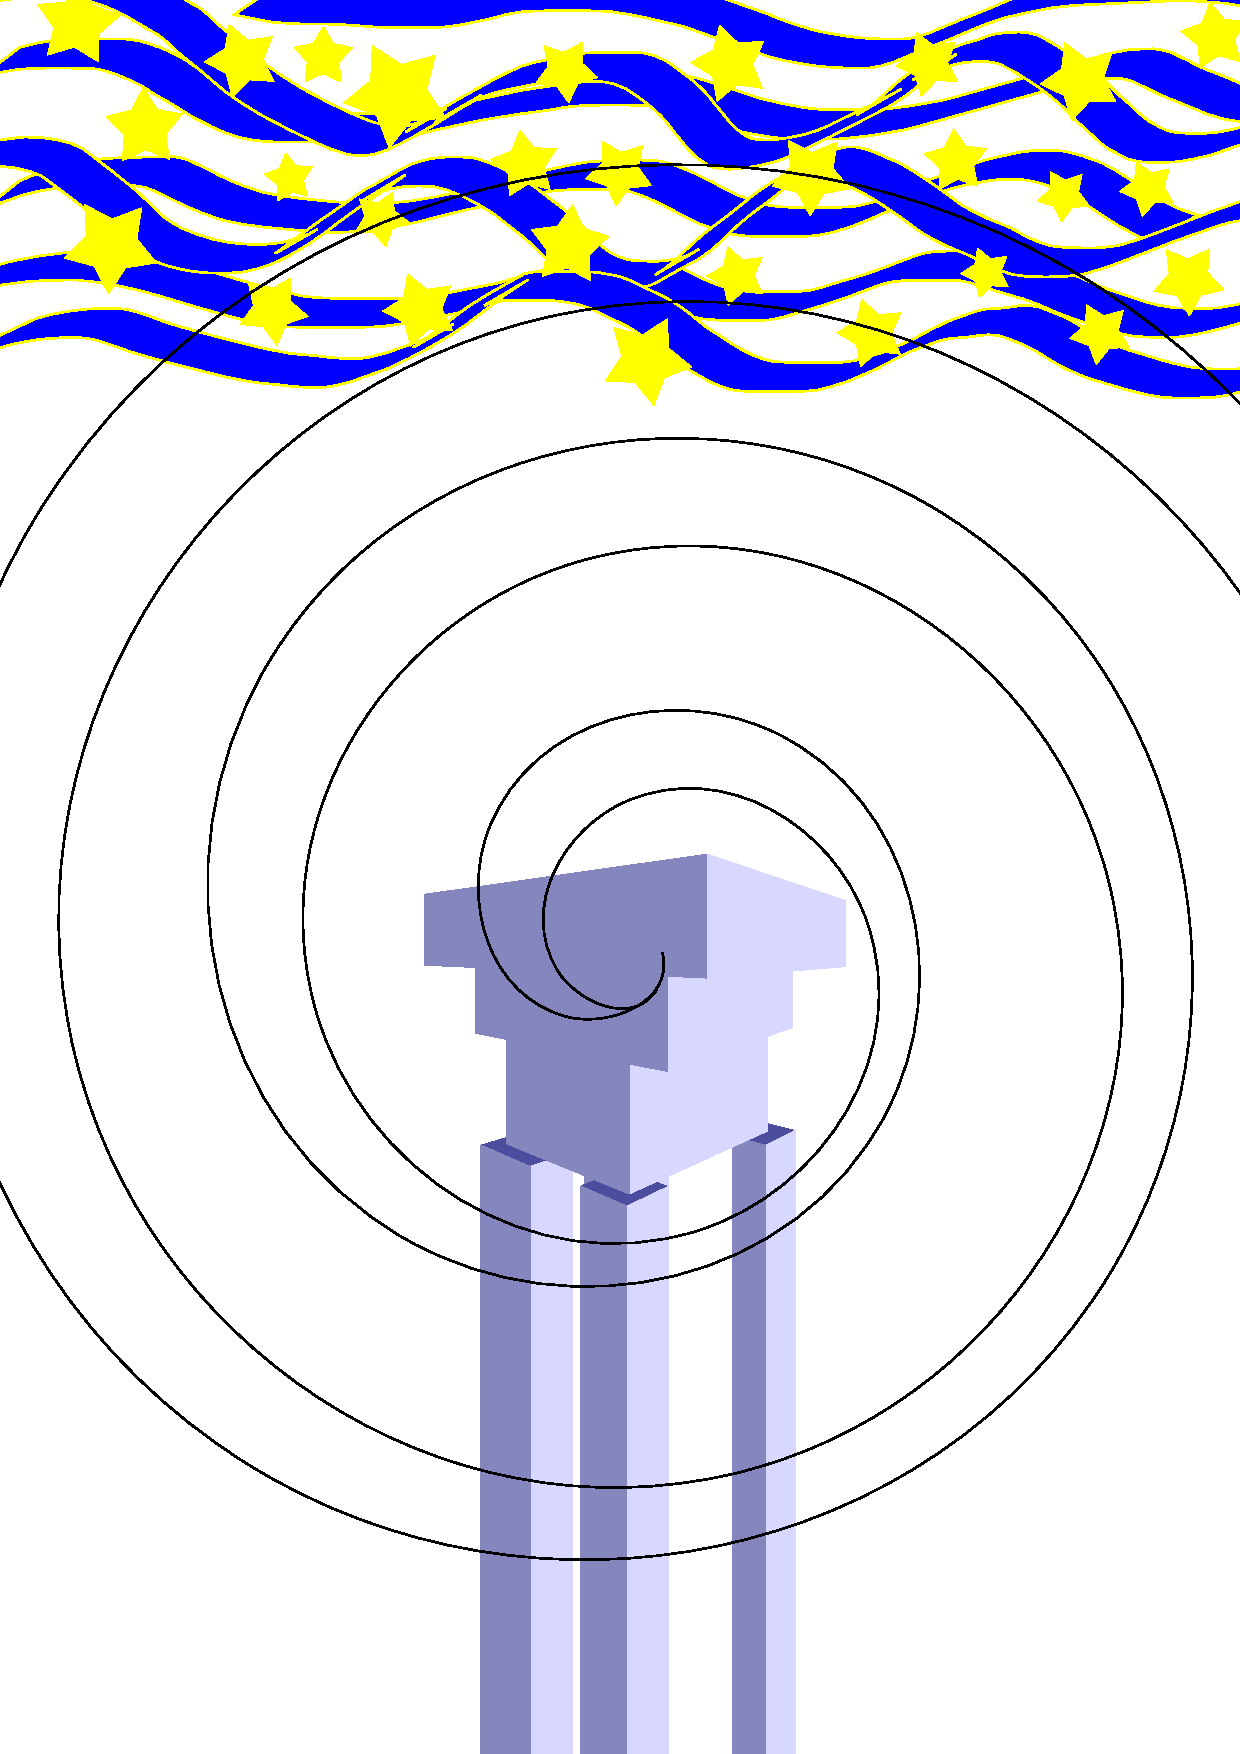
\includegraphics[width=0.75\textwidth]{wektorowa.pdf}
	\caption{Przekaźnik radiowy}
	\label{fig:Przekaźnik radiowy}
\end{figure}

\newpage

\bibliographystyle{abbrv}
\bibliography{Projekt}

\end{large}

\end{document}